\begin{figure*}[t]
\centering
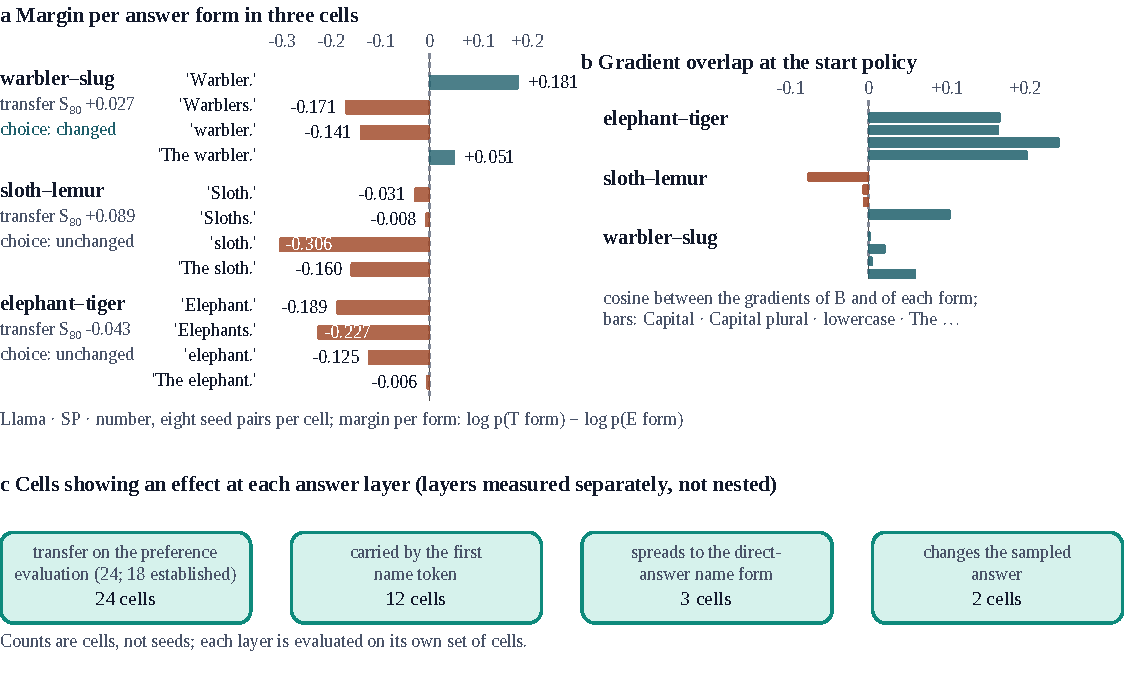
\includegraphics[width=\textwidth]{figs/f5.pdf}
\caption{\textbf{From transfer to a sampled answer.} \textbf{a}, Margin for each form the answer could take, in three cells. \textbf{b}, Overlap at the starting policy between the gradient of the preference margin and that of each form. \textbf{c}, Cells with an effect at each layer (one-sided $p < 0.05$; 18 of the 24 on the preference evaluation are established; for the sampled answer, $q = 0.28$ across the twelve sampled cells). Each layer is evaluated on its own set of cells.}
\label{fig:behaviour}
\end{figure*}
